%%=============================================================================
%% Methodologie
%%=============================================================================

\chapter{Methodologie}
\label{ch:methodologie}

%% TODO: Hoe ben je te werk gegaan? Verdeel je onderzoek in grote fasen, en
%% licht in elke fase toe welke stappen je gevolgd hebt. Verantwoord waarom je
%% op deze manier te werk gegaan bent. Je moet kunnen aantonen dat je de best
%% mogelijke manier toegepast hebt om een antwoord te vinden op de
%% onderzoeksvraag.

\section{Analyse}
Eerst werd een denk-analyse uitgevoerd om te achterhalen welke manieren er waren om de twee projecten met elkaar te laten communiceren.

Aangezien er aanpassingen moesten gebeuren aan het Scratch project omdat een rechtstreekse import niet werkte door het gebrek aan functionaliteit, werd geopteerd om een nieuwe versie van het Scratch project te maken en deze te publiceren op npm. 

Om deze analyse verder uit te voeren werd gekeken naar wat de store van het hoofdproject nodig had als parameters. Daarna werden een reeks methodes uitgeprobeerd om te zien wat wel werkte en wat niet.


\section{Methodes}
\subsection{Functie combineReducers}
In de eerste methode werd geprobeerd om de root reducer van het scratch project rechtstreeks te integreren in de store van het hoofdproject. In de configuratie van de store wordt meegegeven wat de root reducer is en wat de initiële state van de applicatie is. De bedoeling was om een grote gecombineerde root reducer te maken om daarmee de store te initialiseren. Het enige wat hier aangepast werd aan de scratch-integration package was het exporteren van de root reducer in de index file.

Twee root reducers met elkaar combineren via de methode \textit{combineReducers} (figuur 2.1) gaat echter niet zomaar. Deze methode is een functie met als parameter de reducers die moeten gecombineerd worden. Zoals eerder vermeld bevat een reducer een key en een value. De parameter bevat dus een lijst van reducers met elk hun key en value. De functie \textit{combineReducers} overloopt deze lijst en vraagt eerst alle keys op en schrijft deze weg in een nieuwe variabele. Daarna wordt voor elke reducer key gekeken of de corresponderende value een functie is. Als dit zo is, dan wordt deze reducer weggeschreven in een nieuwe lijst variabele.   

Deze functie retourneert dan opnieuw een functie 'combination'. In de scope van deze functie zitten onder andere twee lijsten. Een lijst voor de finale reducer keys en een lijst voor de finale reducers. 
 
Omdat deze na combinatie in de scope van de functie zitten, is het onmogelijk om na een eerste combinatie een tweede combinatie uit te voeren. Dit zorgt er dus voor dat eenmaal er een root reducer gecombineerd is, deze niet opnieuw kan gebruikt worden om nog eens te combineren met een andere root reducer. Om hier verder op in te spelen werd naar een tweede methode gezocht. 

\subsection{Eigen methode}
Als tweede methode werd gezocht naar een alternatief. De bedoeling van deze extensie zou als het ware een uncombineReducers methode zijn. Op deze manier kan snel alles los gemaakt worden van elkaar om dan later opnieuw te kunnen combineren. Op deze manier kan ook een lineaire structuur verkregen worden. Momenteel is het niet mogelijk om van reeds gecombineerde root reducers een nieuwe reducer te combineren met behoud van functionaliteit van beide root reducers en een lineaire structuur in plaats van een geneste structuur. 

\paragraph{Analyse}
Om een extensie te schrijven is er een duidelijk inzicht nodig in de methode combineReducers (figuur 2.1). Hiervoor werd dus eerst een analyse gedaan van deze methode.
\begin{figure}
	\begin{center}
		\caption{Methode combineReducers uit de Redux package. Verkregen van \textcite{Redux01}}
		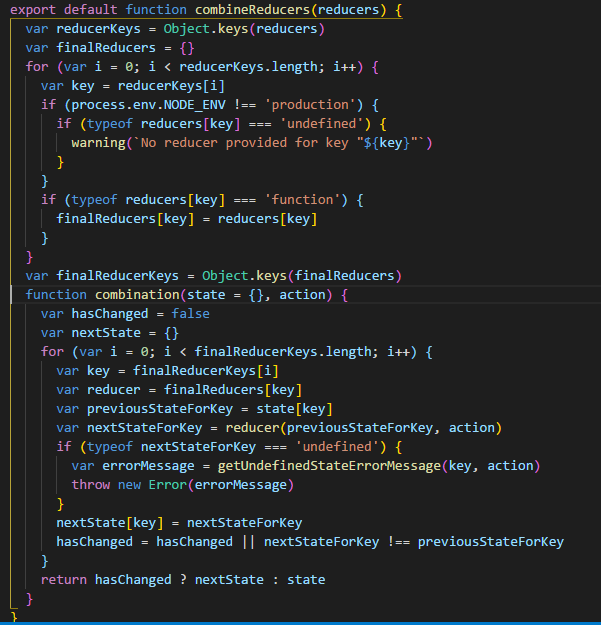
\includegraphics[width=14cm]{img/combineReducers}\\[0.5cm]
	\end{center}
\end{figure} 

De methode neemt reducers als parameter. Er worden eerst twee lokale variabelen gemaakt, de reducerKeys met daarin de keys van de reducers die als parameter werden meegegeven en de finalReducers. Daarna wordt -zolang er reducerKeys zijn- de juiste reducer opgehaald aan de hand van zijn key en wordt er gekeken als het type een functie is of niet. Als het inderdaad een functie is dan zal deze worden opgeslaan in de finalReducers.

Nu kan er een nieuwe variabele finalReducerKeys aangemaakt worden met daarin de keys van de finalReducers. Daarna wordt er een functie geretourneerd met dezelfde syntax als de reducer (state en action). Er wordt opnieuw per key overlopen, deze keer om een object te verkrijgen via \textit{reduce} aan de hand van de state voor deze key.

\paragraph{Werkwijze}

Bij een reducer die voor de eerste keer gecombineerd wordt (figuur 2.1), zal door de functie \textit{object.keys} elke key aangesproken worden. Hierdoor zal elke reducer opgenomen worden in de combinatie. Wanneer een combinatie tracht gemaakt te worden van een reeds gecombineerde reducer, dan zal door de functie \textit{object.keys} enkel de gecombineerde key aanspreken en dus niet alle onderliggende reducers. Er werd getracht om van een root reducer, die reeds gecombineerd is, de reducer keys aan te spreken van zijn onderliggende reducers. Omdat deze reducers al eens gecombineerd zijn, zitten deze onderliggende reducers in de scope van de functie combineReducers. Daardoor is het niet mogelijk om van een gecombineerde reducers opnieuw zijn reducers aan te spreken, deze kunnen niet worden aangesproken. Indien dit wel mogelijk zou zijn, kon op deze manier een lineaire combinatie gemaakt worden van meerdere root reducers. 

Omdat dit niet mogelijk is, wordt de functionaliteit van onderliggende reducers niet meegenomen. Dit zorgt er dan weer voor dat deze reducers niet opgenomen worden in de state. Vanaf het moment dat een reducer nodig zou zijn om functionaliteit af te handelen, zal de app crashen omdat het een undefined reducer zal oproepen. 

Om hier een oplossing voor te bieden werd gekeken naar een alternatief voor de methode combineReducers. 
Er werd geprobeerd om geen rechtstreeks gebruik te maken van de root reducer van Scratch, maar om alle reducers te combineren in een groot object en dan dat object te exporteren. Om deze methode mogelijk te maken moet de root reducer van het hoofdproject ook een object zijn en geen gecombineerde functie. Een voorbeeld kan gevonden worden in (zie figuur 2.2). Anders keert het probleem van de function scope terug. Met beide root reducers als object is het wel mogelijk om een gecombineerde root reducer af te leveren. De lijsten van de reducer keys en reducers bevatten dan de keys en reducers van beide projecten. Hierdoor wordt dus de volledige functionaliteit omvat van beide projecten.

\begin{figure}
	\begin{center}
		\caption{Object export methode in plaats van combineReducers}
		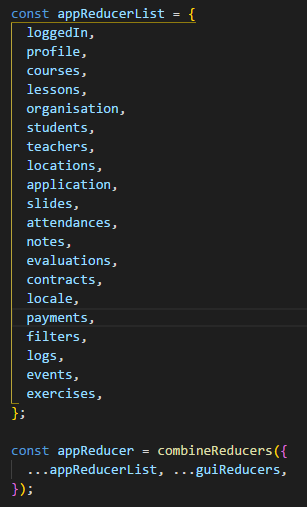
\includegraphics[width=8cm]{img/combineReducers-object-export}\\[0.5cm]
	\end{center}
\end{figure}
 
\subsubsection{Nadelen}
Een eerste nadeel van deze methode is dat er dan ook met de root reducer van het hoofdproject rekening moet gehouden worden. Deze mag dan namelijk ook niet gecombineerd zijn. Om deze methode uit te voeren was er een gedeeltelijke herstructurering nodig, waardoor deze methode al niet meer optimaal is. 

Een tweede nadeel zijn de veranderingen in het Scratch project. Stel dat er een reducer bijkomt of verwijderd wordt, dan moet dit altijd manueel aangepast worden vooraleer er terug een werkende versie geproduceerd wordt. Indien er enkel nood is aan de root reducer die geëxporteerd wordt, dan zou dit geen probleem zijn aangezien deze veranderingen mee opgenomen worden in de combinatie van de root reducer. Door elke reducer afzonderlijk in een nieuw object te steken en zo te exporteren wordt er heel wat extra onderhoudswerk gecreëerd voor deze package.  

Een derde nadeel zijn de configuraties en dependencies die nodig zijn om het Scratch project te laten draaien. 
Elke dependency die gebruikt wordt, moet ook mee overgenomen worden in de package.json van het hoofdproject. Dit zorgt ervoor dat de configuraties van webpack ook moeten meegenomen worden. Om dit te realiseren werd een nieuwe package gemaakt van de bestaande react-scripts package met de uitbreidingen die nodig zijn om een succesvolle integratie te verkrijgen.

Dit derde nadeel kan echter wel opgelost worden. Via webpack is het mogelijk om de configuraties van Scratch te bundelen en weg te schrijven in een dist map om zo te exporteren als een library. In dit geval gaat het pas gebeuren wanneer de environment variabele op 'production' staat. Een tweede package op npm met de nodige configuraties voor beide projecten wordt overbodig wanneer deze oplossing gebruikt wordt in de package waar de reducers geëxporteerd worden. Dit bespaart onderhoudswerk en vermindert de complexiteit.

Om deze oplossing te testen werd gebruik gemaakt van een aantal objectieve methodes om de complexiteit te bepalen. Eerst werd er gekeken naar de Halstead complexiteitsmeting. Deze metriek houdt rekening met de volume (lines of code) van de applicatie, alsook de moeilijkheid en de inspanning die geleverd moet worden. Als resultaat van deze metriek werd geconcludeerd dat er weinig inspanning moet geleverd worden en dat de oplossing een lage complexiteit heeft. 

Ten tweede werd er gekeken naar de cyclomatische complexiteit van de oplossing. Deze metriek kijkt naar het aantal lineair onafhankelijke paden doorlopen worden door de oplossing. Gezien het gaat om een lineaire oplossing kon er hier ook vrij snel geconstateerd worden dat er een lage complexiteit is volgens deze metriek. 

De laatste objectieve methode is de maintainability index. Deze is een combinatie van voorgaande metrieken. Op basis van de maintainability index alleen kan geen oordeel geveld worden. Een hoge maintainability index wil niet rechtstreeks zeggen dat er een goeie onderhoudbaarheid is en dat het programma een lage complexiteit heeft. Er kan namelijk een hoge maintainability index verkregen worden met een slechte waarde voor de cyclomatische complexiteit en een goeie voor de Halstead metriek of omgekeerd. Gezien voorgaande complexiteitsmetingen reeds positief waren kan er hier ook de conclusie getrokken worden dat het gaat om een weinig complexe, goed onderhoudbare oplossing.


